\section{Lecture 22: The Harmonic Oscillator with Angular Momentum} 

Recall that the Hamiltonian of the Harmonic Oscillator
\[ \hat{H} = \frac{\hat{p}^2}{2m} + \frac{1}{2} m \omega^2 \hat{x}^2 \]
Solving this in Cartesian coordinates gives 3 independent differential equations with solution:
\[ \Psi_n \sim e^{-x^2} H_n(x) \]
But let's take an operator perspective. Recall the raising and lowering operators:
\[ \hat{a}_{\pm} = \frac{1}{\sqrt{2}} \qty(\qty(\frac{m\omega}{\hbar})^{1/2} \mp \frac{i \hat{p}_x}{(m \hbar \omega)^{1/2}}) \]
These act on the energy eigenstates by doing:
\begin{align*}
    \hat{a}_{+} \ket{\Psi_n} &= \sqrt{n + 1} \ket{n + 1} \\
    \hat{a}_{-} \ket{\Psi_n} &= \sqrt{n} \ket{n - 1}
\end{align*}

We can draw parallels with the angular momentum operator.
\begin{align*}
    L_x &= y p_z - z p_y \\
    L_y &= z p_x - x p_z \\
    L_z &= x p_y - y p_x
\end{align*}

We derived last time the simultaneous eigenfunctions of $ \hat{L}^2, \hat{L}_z $
as $\Psi_{\ell m} \sim Y_{\ell m}(\theta, \varphi)$. This is how the operators act:
\begin{align*}
    \hat{L}^2 \ket{\ell m} &= \ell (\ell + 1) \hbar^2 \ket{\ell m} \\
    \hat{L}_z \ket{\ell m} &= m \hbar \ket{\ell m}
\end{align*}

Now let's develop some ladder operators:
\[ \hat{L}_{\pm} = \hat{L}_x \pm i \hat{L}_y \]
this is our guess--let's see how they interact.
\begin{align*}
    [\hat{L}^2, \hat{L}_{\pm}] &= 0 \\
    \hat{L}_{\pm} \hat{L}_{\mp} &= \hat{L}_x^2 + \hat{L}_y^2 \pm \hbar \hat{L}_z = \hat{L}^2 - \hat{L}_z^2 \pm \hbar \hat{L}_z \\
    [\hat{L}_+, \hat{L}_{-}] &= 2\hbar \hat{L}_z \\
    [\hat{L}_z, \hat{L}_{\pm}] &= \pm \hbar \hat{L}_{\pm} \\
\end{align*}

Let's try applying the operator now:
\begin{align*}
    \hat{L}_z \ket{\ell m} &= m \hbar \ket{\ell m} \\
    \hat{L}_{\pm} \hat{L}_z \ket{\ell m} &= \hat{L}_{\pm}(m \hbar \ket{\ell m}) \\
    (\hat{L}_z \hat{L}_{\pm} \mp \hbar \hat{L}_{\pm}) \ket{\ell m} &= m \hbar \hat{L}_{\pm} \ket{\ell m} \\
    \hat{L}_z \hat{L}_{\pm} &= (m \pm 1) \hbar \hat{L}_{\pm} \ket{\ell m}
\end{align*}
So, the raising/lowering operator increases/decreases the eigenvalue by $\hbar$. This means the $z$ projection of the vector is changed.

Further,
\begin{align*}
    \hat{L}^2 \ket{\ell m} &= \ell (\ell + 1)\hbar^2 \ket{\ell m} \\
    \hat{L}_{\pm} \hat{L}^2 \ket{\ell m} &= \ell (\ell + 1) \hbar^2 \hat{L}_{\pm} \ket{\ell m} \\
    \hat{L}^2 \hat{L}_{\pm} \ket{\ell m} &= \ell (\ell + 1) \hbar^2 \hat{L}_{\pm} \ket{\ell m}
\end{align*}
This raising/lowering does not change the total angular momentum. Since the $z$ component was changed but the total length was not changed, this is just
an orientation change of the momentum. There is also normalization which we can omit. We can summarize this as:
\begin{theorem}
    The raising and lowering operators for the $z$ component angular momentum act as:
    \[ \hat{L}_{\pm} \ket{\ell m} = \hbar [\ell(\ell + 1) - m (m \pm 1)]^{1/2} \ket{\ell, m \pm 1}\]
\end{theorem}
Note we can also write $\hat{L}_x$ in terms of the raising/lowering:
\begin{align*}
    \hat{L}_x &= \frac{1}{2} \qty(\hat{L}_+ + \hat{L}_-) \\
    \hat{L}_y &= \frac{1}{2i} \qty(\hat{L}_+ - \hat{L}_-)
\end{align*}
But now we find the average position:
\begin{align*}
    \langle L_x \rangle &= \bra{\ell m} \hat{L}_x \ket{\ell m} \\
    &= \frac{1}{2} \bra{\ell m} \hat{L}_+ + \hat{L}_- \ket{\ell m} \\
    &= 0
\end{align*}
Similarly $\langle L_y \rangle = 0$. But we think that the actual angular momentum shouldn't be identically 0.
We check the expectation of its square:
\begin{align*}
    \langle L_x^2 \rangle &= \langle L_y^2 \rangle = \frac{1}{2} \langle L^2 - L_z^2 \rangle \\
    &= \frac{1}{2} \qty(\ell (\ell + 1) - m^2) \hbar^2
    &\geq \frac{\ell \hbar^2}{2}
\end{align*}
Even when you have maximum $z$ component, $m^2 = \ell^2$, there is still a piece of the vector in other directions!
To avoid violating Heisenberg uncertainty, the vector is still a bit longer than the $z$ component.

For example take the case of $\ell = 2$. We know $m \in \{-2, -1, 0, +1, +2\}$. Note that: $|L| = \sqrt{6} \hbar$.
We can then plot different vectors for different values of $m$.

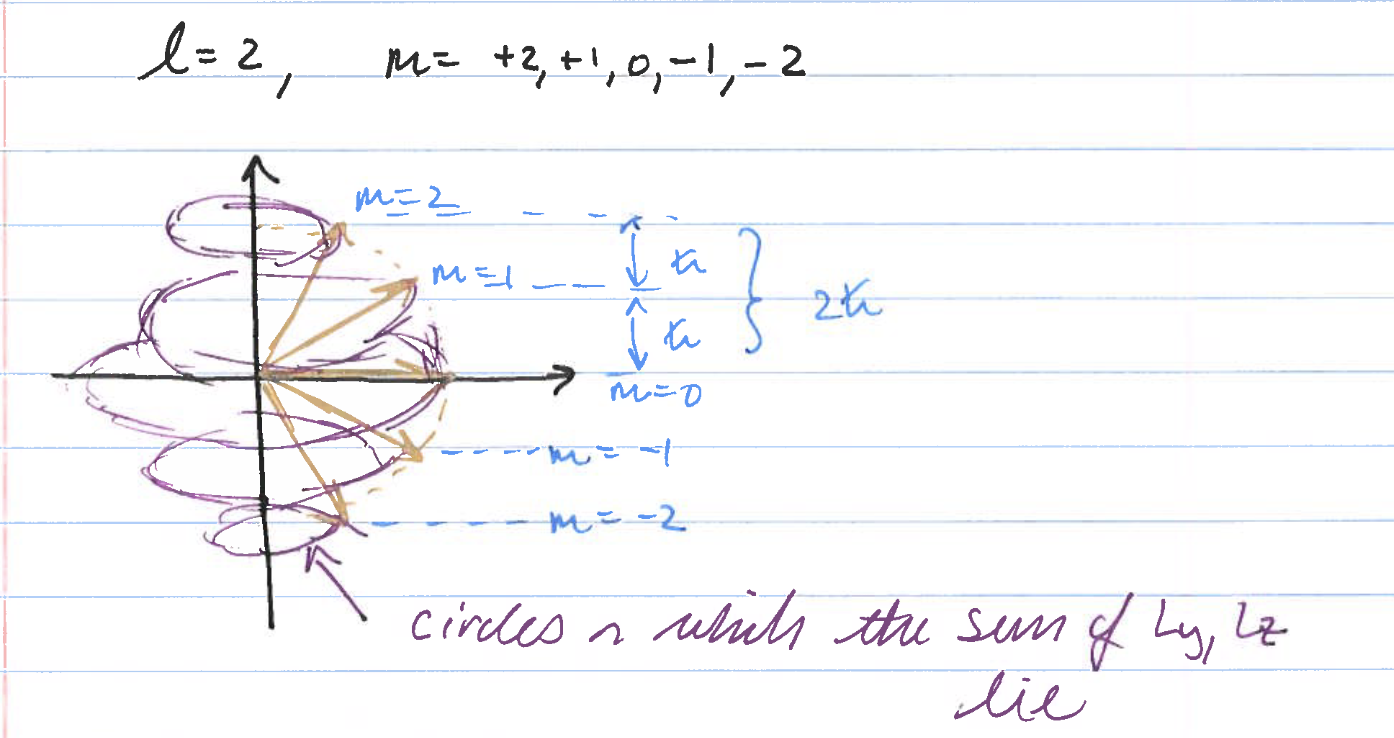
\includegraphics[width=300px]{angs.png}

Consider a particle of mass $\mu$. The kinetic energy is:
\begin{align*}
    \hat{T} = \frac{\hat{p}^2}{2 \mu} \\
    &= -\frac{\hbar^2}{2\mu} \nabla^2 \\
    &= -\frac{\hbar^2}{2\mu} \qty(\frac{1}{r^2} \pdv{}{r} \qty(r^2 \pdv{}{r}) + \frac{1}{r^2 \sin \theta} \pdv{}{\theta} \qty(\sin \theta \pdv{}{\theta}) + \frac{1}{r^2 \sin^2 \theta} \pdv{}{\varphi^2}) \\
    &= -\frac{\hbar^2}{2\mu} \qty(\frac{1}{r^2} \pdv{}{r} \qty(r^2 \pdv{}{r}) - \frac{\hat{L}^2}{\hbar^2 r^2})
\end{align*}
If we constrain the particle to live on sphere of $r = a$:
\begin{align*}
    \hat{T} &=\frac{\hat{L}^2}{2 \mu a^2} \\
    &= \frac{\hat{L}^2}{2I}
\end{align*}
where $I$ is the moment of inertia. Thus:
\begin{align*}
    \hat{H} &= \frac{\hat{L}^2}{2I} + \hat{V}(\theta, \varphi)
\end{align*}

The simplest problem is that of the rigid rotor, when $\hat{V} = 0$.
\begin{align*}
    \hat{H} &= \frac{\hat{L}^2}{2I} \implies E_{\ell} = \frac{\hbar^2}{2\pi} \ell (\ell + 1)
\end{align*}
This immediately gives you the rotation energy of diatomic molecules.
